%\documentclass[12pt,handout]{beamer}
\documentclass[presentation]{beamer}
\usepackage{../oop-slides-lab}
\setbeamertemplate{bibliography item}[text]

\newcommand{\lab}{Lab01}

\title[{\lab} -- Introduzione]{Introduzione al laboratorio}

\date[\today]{\today}

\begin{document}

\frame[label=coverpage]{\titlepage}

\begin{frame}<beamer>
	\frametitle{Outline}
	\tableofcontents[]
\end{frame}

\section{Organizzazione del Laboratorio}\label{sec:organizzazione-del-laboratorio}

\begin{frame}{Organizzazione del Laboratorio}
    \begin{itemize}
        \item Due turni settimanali
        \begin{itemize}
            \item Per esigenze di spazi, per garantire un maggiore supporto ai frequentanti, \dots
        \end{itemize}
        \item Il contenuto della lezione e dell'esecitazione settimanale del laboratorio è il medesimo per entrambi i turni
        \item La gestione della partecipazione ai turni è demandata al prof. Viroli
        \item Nello stesso giorno avrete sia OOP che OS
    \end{itemize}
    \begin{block}{Primo Turno}
        \begin{itemize}
            \item Lunedì, 9:00 - 13:00
            \item Lab. 2.2, Campus Cesena
        \end{itemize}
    \end{block}
    \begin{block}{Secondo Turno (cognomi nell'intervallo [Gin-Z])}
        \begin{itemize}
            \item Martedì, 14:00 - 18:00
            \item Lab. 2.2, Campus Cesena
        \end{itemize}
    \end{block}
\end{frame}

\begin{frame}{Turni e app ``Presente''}
    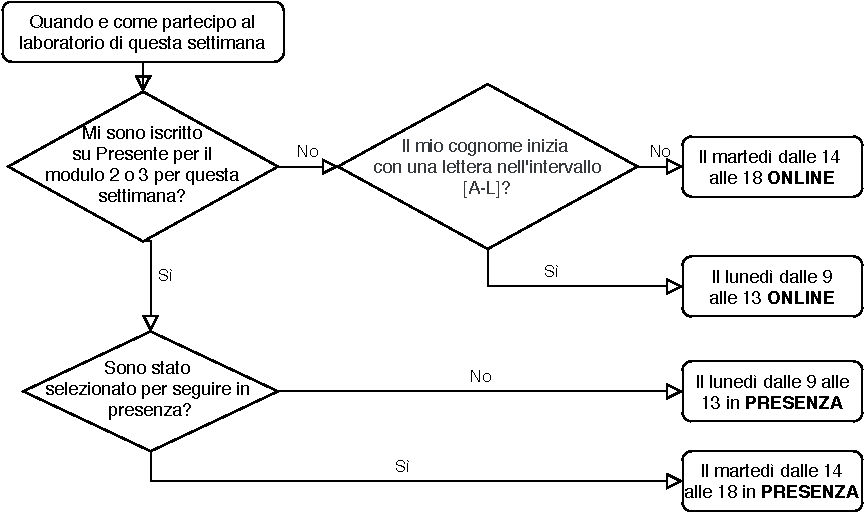
\includegraphics[width=\textwidth]{covid-presente}
\end{frame}

\begin{frame}{Docenti del Laboratorio}
    \begin{block}{Prof. Danilo Pianini -- Responsabile Modulo 1}
        \begin{itemize}
            \item mail: \texttt{danilo.pianini@unibo.it}
            \item ricevimento: Martedì, 17:00 - 18:00
        \end{itemize}
    \end{block}
    \begin{block}{Prof. Roberto Casadei -- Responsabile Modulo 2}
        \begin{itemize}
            \item mail: \texttt{roby.casadei@unibo.it}
            \item ricevimento: su appuntamento, da concordare via mail
        \end{itemize}
    \end{block}
    \begin{block}{Ing. Andrea Placuzzi -- Tutor Didattico}
        \begin{itemize}
            \item mail: \texttt{andrea.placuzzi@unibo.it}
        \end{itemize}
    \end{block}
    \begin{block}{Ing. Niccolò Maltoni -- Tutor Didattico}
        \begin{itemize}
            \item mail: \texttt{niccolo.maltoni@unibo.it}
        \end{itemize}
    \end{block}
\end{frame}

\section{Forum e supporto}

\begin{frame}{Chiarimenti e spiegazioni}

Per chiarimenti, ulteriori delucidazioni e spiegazioni fuori dall'orario di laboratorio
si incoraggia l'uso del \textbf{Forum del Corso}
\begin{itemize}
    \item link accessibile dal sito del corso su Virtuale
    \item da preferire all'email inviata direttamente al/ai docente/i
\end{itemize}

\begin{block}{}
    \begin{itemize}
        \item Il dubbio di uno studente, probabilmente, è anche il dubbio di qualcun'altro (\textbf{condivisione})
        \item Gli studenti possono aiutarsi (\textbf{discussione})
        \item Aiutare i colleghi sul forum è \textbf{valutato positivamente}
    \end{itemize}
\end{block}
\vfill
\begin{itemize}
\item L'email resta il canale da utilizzare per comunicazioni \textbf{confidenziali}
    \begin{itemize}
        \item con l'accortezza di mettere sempre in copia \emph{tutti} i docenti del corso
    \end{itemize}
\end{itemize}



\end{frame}

\begin{frame}{Il Laboratorio}

\begin{itemize}
    \item Consente di mettere in pratica quanto visto nelle lezioni in aula
    \begin{itemize}
        \item con il supporto diretto del docente e del tutor
    \end{itemize}
    \item Integra ed espande i contenuti affrontati in aula
    \item Introduce \textbf{nuovi} strumenti e metodologie (non affrontati in aula!)
    \begin{itemize}
        \item Strumenti, metodologie, pratiche, librerie\dots{}
    \end{itemize}
\end{itemize}

\begin{block}{Organizzazione di ciascun turno di laboratorio}
    \begin{enumerate}
        \item Lezione Frontale (30-60 min)
        \begin{itemize}
            \item Introduce \textbf{nuovi concetti} non visti in aula
        \end{itemize}
        \item Esercitazione
        \begin{itemize}
            \item Un set di esercizi da svolgere in autonomia
            \item Evocando il docente in caso di difficoltà
            \item Chiedendo \textbf{sempre} ai docenti una \textbf{correzione finale}
        \end{itemize}
    \end{enumerate}
\end{block}
\end{frame}

\begin{frame}{Svolgimento di ciascun esercizio}
    \begin{enumerate}\itemsep20pt
        \item Lettura della consegna
        \begin{itemize}
            \item Contattare un docente in caso di dubbi
        \end{itemize}
        \item Svolgimento dell'esercizio
        \begin{itemize}
            \item Contattare un docente in caso di difficoltà
        \end{itemize}
        \item \textbf{Segnalazione al docente/tutor del avvenuto completamento}
        \begin{itemize}
            \item \textit{La correzione è fondamentale!}
            \item Nella correzione, progressivamente, vi verranno dati suggerimenti per passare da "qualcosa che funziona"
            a qualcosa di ben fatto!
            \item Ricordate che in OOP \textit{``funziona'' non è una metrica di qualità sufficiente}
        \end{itemize}
    \end{enumerate}
\end{frame}

\begin{frame}{Come chiedere supporto ai docenti}
    A causa della didattica mista, quest'anno sperimenteremo un approccio nuovo:
    \begin{itemize}
        \item Ciascuno studente, che sia in didattica frontale o mista, si prenota tramite un post sul canale Teams corretto
        \item Il docente lo contatta e
        \begin{itemize}
            \item lo raggiunge fisicamente se presente
            \item Apre una call privata (se remoto)
        \end{itemize}
    \end{itemize}
    \begin{block}{Canale per informazioni}
        \begin{itemize}
            \item \textbf{URL}: \url{http://bit.ly/oop-2020-info}
            \item Da usare per domande, spiegazioni, chiarimenti
        \end{itemize}
    \end{block}
    \begin{block}{Canale per le correzioni}
        \begin{itemize}
            \item \textbf{URL}: \url{http://bit.ly/oop-2020-correzioni}
            \item Ad ogni esercizio terminato, ogni studente \textbf{deve} prenotarsi per far correggere quanto fatto
        \end{itemize}
    \end{block}
\end{frame}


\section{Contenuti e Obiettivi}

\begin{frame}{Overview sui contenuti}

\begin{enumerate}
    \item Tooling Java
    \item Eclipse IDE, debug tools
    \item Controllo di versione
    \item Testing, documentazione, deployment
    \item Controllo di qualità del codice
    \item Programmazione multipiattaforma
    \item Profiling
    \item JavaFX
    \item C\# IDE e tools
\end{enumerate}

\end{frame}

\begin{frame}{Obiettivi del Laboratorio}
    \begin{itemize}
        \item Acquisire le completenze necessarie per:
        \begin{enumerate}
            \item diventare ottimi programmatori
            \item diventare discreti progettisti
        \end{enumerate}
        \item Fondamentale: \textbf{mettersi in gioco!}
        \begin{itemize}
            \item specialmente per chi ha già rudimenti di OOP o di Java
            \item il livello è un altro rispetto a quello che potete aver visto alle superiori
            \item percorso a difficoltà crescente
            \begin{itemize}
                \item Il codice passerà in inglese
                \item Le istruzioni passeranno in inglese
                \item Richiederemo sempre maggior qualità
                \item Useremo strumenti via via più avanzati
            \end{itemize}
        \end{itemize}
        \item Fondamentale: \textbf{impegno!}
        \begin{itemize}
            \item È uno dei corsi più ``tosti'' del percorso di studi
            \begin{itemize}
                \item Richiede attenzione in aula
                \item Richiede attenzione e impegno in laboratorio
                \item Richiede studio e pratica a casa
                \item \dots{}duro recuperare se si resta indietro!
            \end{itemize}
        \end{itemize}
    \end{itemize}
\end{frame}

\end{document}

\begin{frame}[allowframebreaks]
 \frametitle{Bibliography}
	\bibliographystyle{plain}
	\small
 \bibliography{biblio}
\end{frame}

